\clearpage
\section{方向光的级联阴影与半影}

下图使用同一台游戏相机。左下方的支墩贴着地面，中间的薄板悬在地面上方 $2.2$ 米。把太阳的角半径从 $0^\circ$ 调到 $4^\circ$，薄板的影子明显变软，支墩脚下的轮廓仍贴着物体。为看清直射光的变化，这一组关闭间接光，使用相同的曝光。$4^\circ$ 用于展示差别，面板初值为 $0.27^\circ$。

\begin{center}
\panelimage{.485\linewidth}{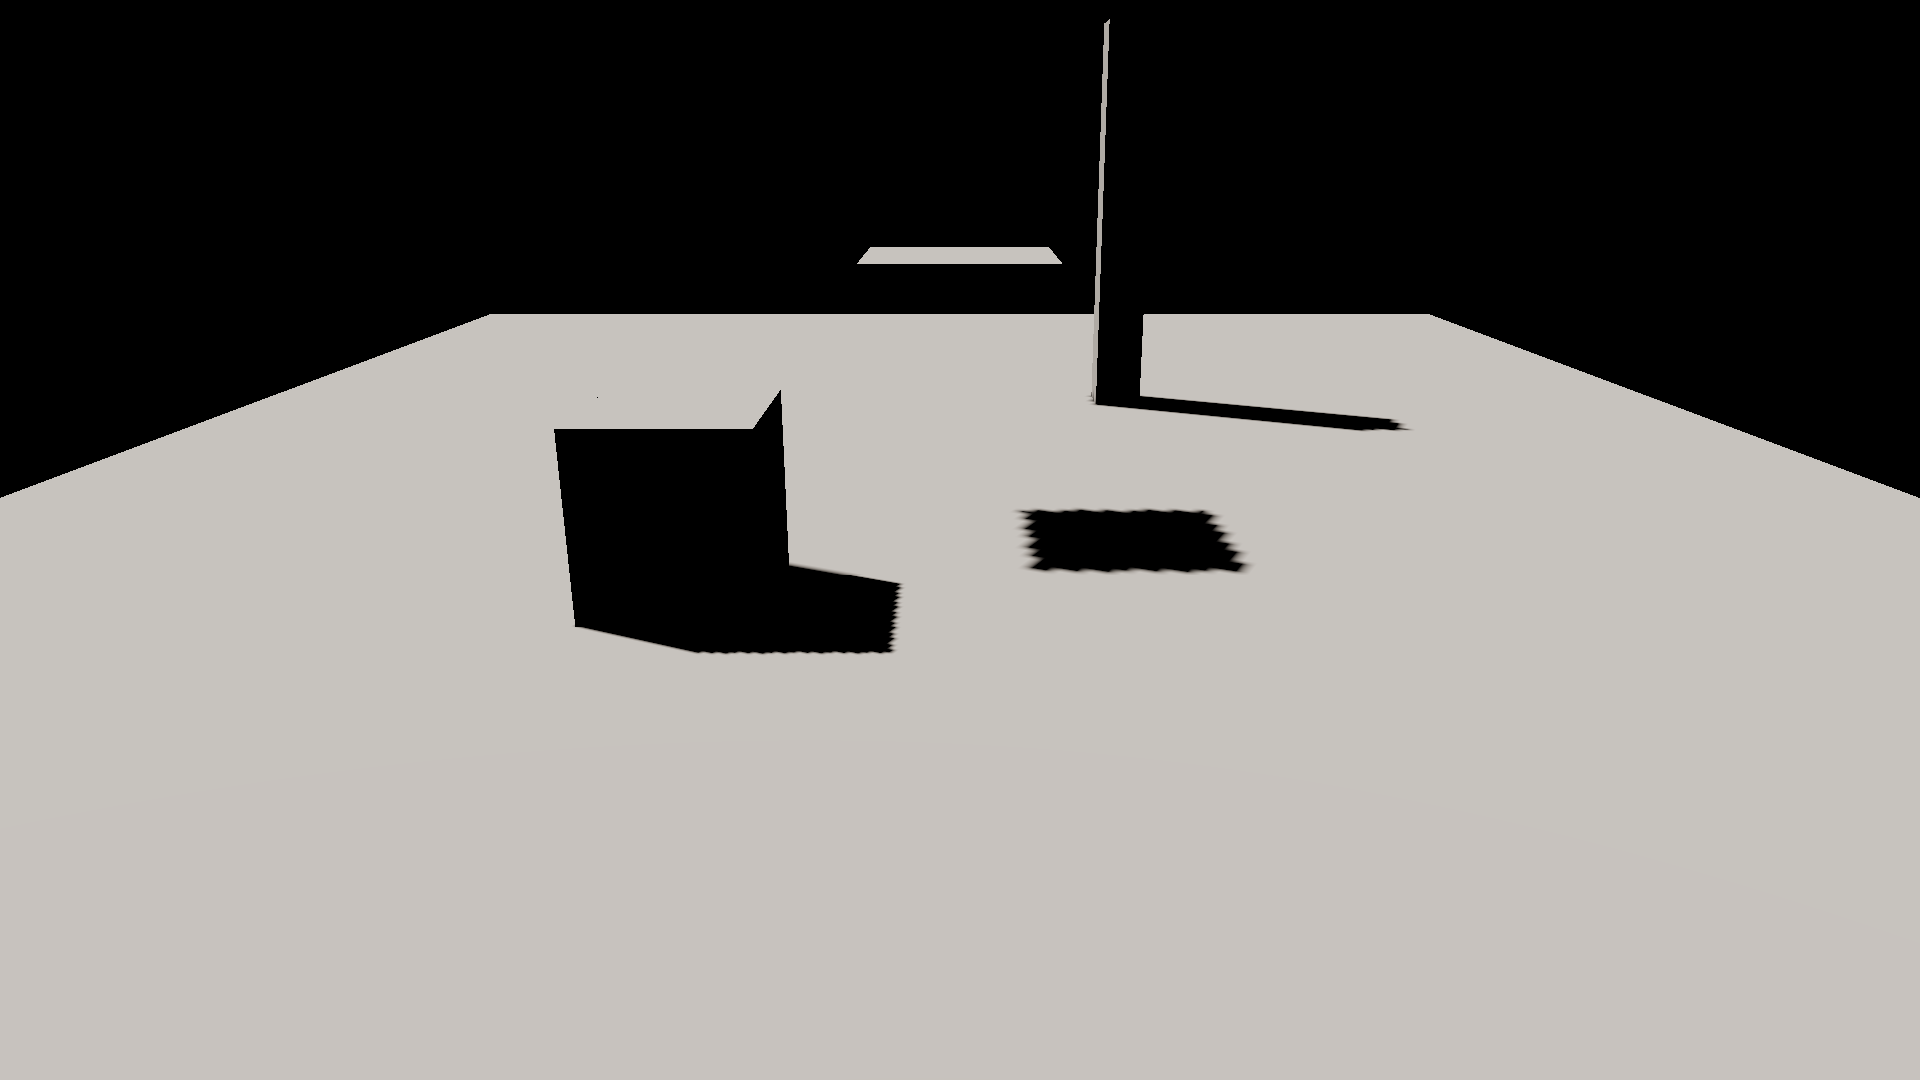
\includegraphics[width=\linewidth]{../../../output/validation/cascaded-shadows/hard.png}}{太阳角半径 $0^\circ$。观察薄板右下方的影子。}\hfill
\panelimage{.485\linewidth}{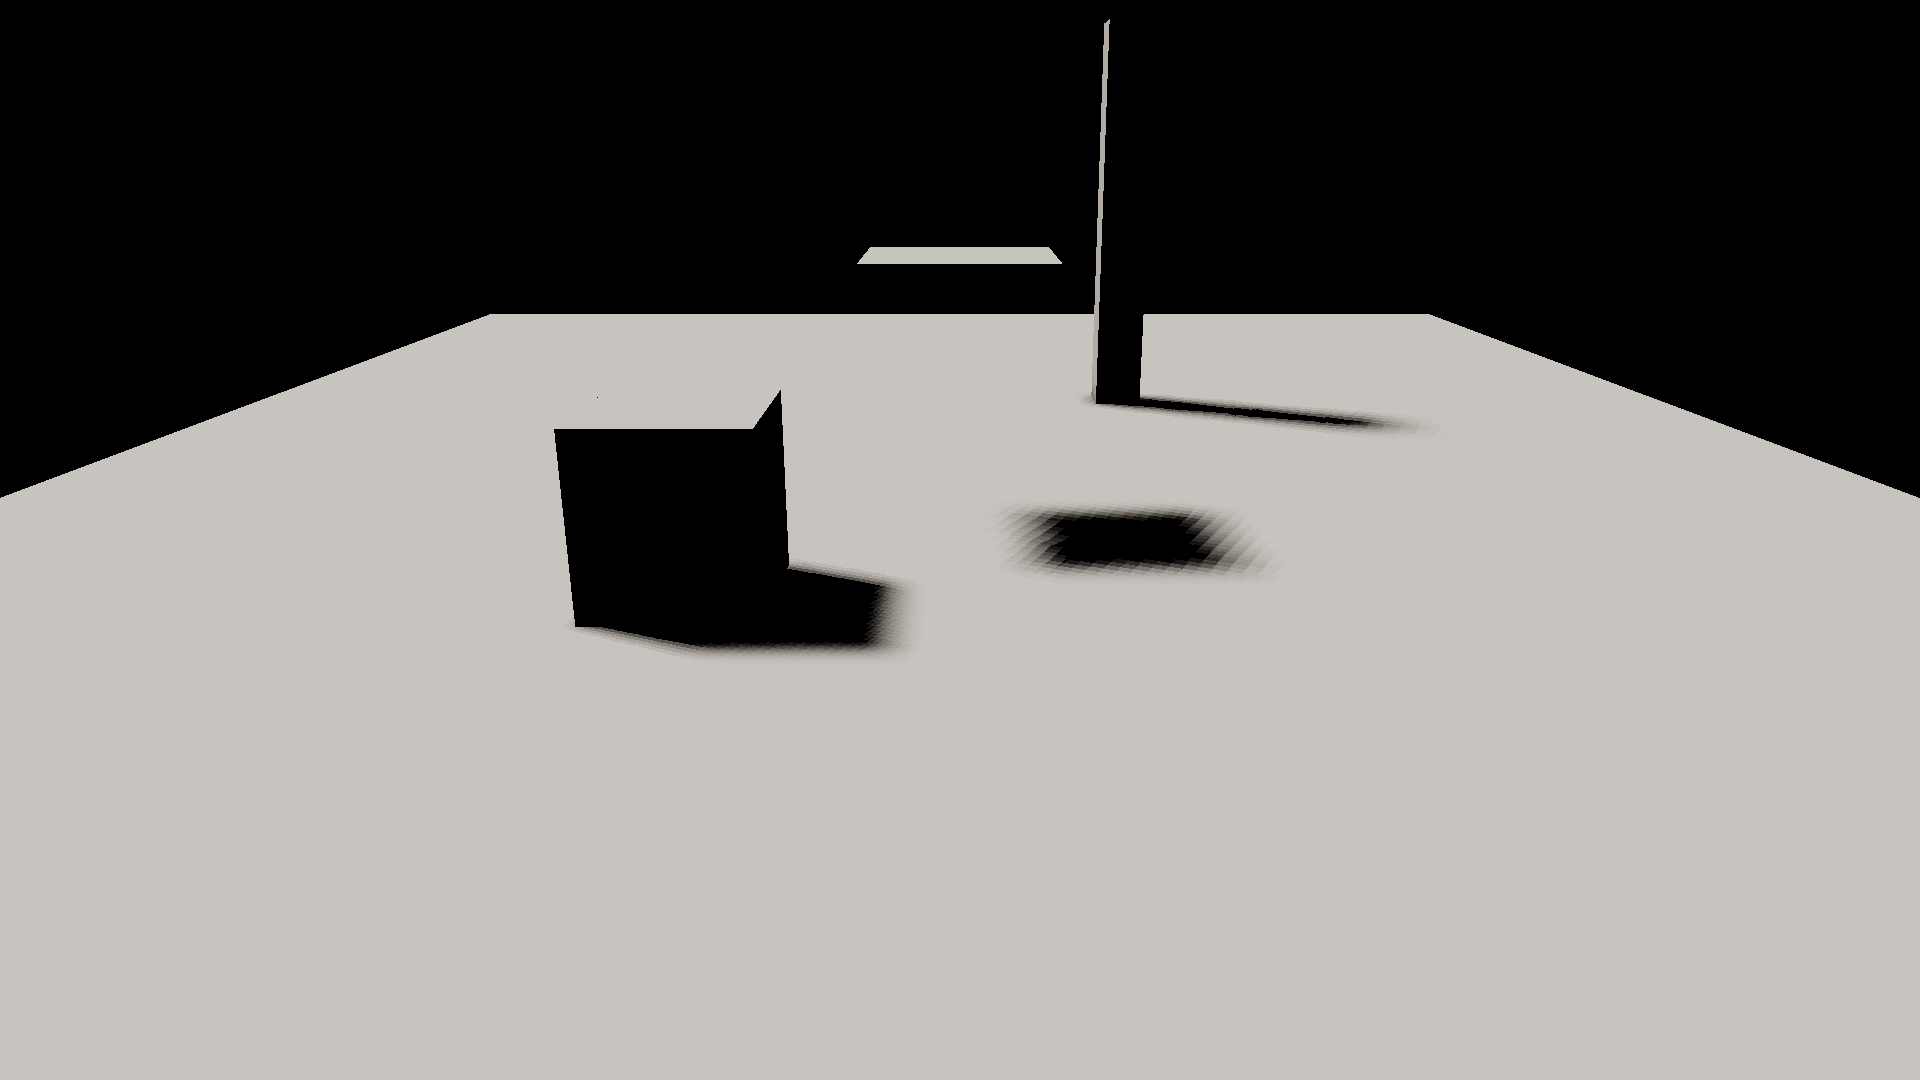
\includegraphics[width=\linewidth]{../../../output/validation/cascaded-shadows/soft.png}}{同机位，$4^\circ$。远处立柱也有一条渐淡的影子。}
\end{center}

游戏相机前方的近、中、远三段各用一张 $512\times512$ 深度图。每张图保存从太阳方向看去最先遇到的表面。近处一张图只负责较小范围，因此地上一米能分配到更多像素。\code{BuildShadowCascades} 按相机距离分段，并把每张图的中心对齐到整格。选定一层后，\code{cascadeVisibility} 从对应深度图中判断地面能见到多少阳光。投影距离限制在 $24$ 米，超过后直接光照不再查询这些图。配置入口是 Vulkan 场景视图“实时效果”里的“级联阴影 CSM”。层数设为 0 即回到原场景的阴影方式。

设悬板离地 $h$ 米。对于正照下来的太阳，最外缘的光线偏离中心方向 $\alpha$。把这条光线、竖直高度和地面画成直角三角形，地面上的横向距离就是 $h\tan\alpha$。这给出从影子边缘向一侧扩展的半宽。夹具把一块挡板举到离地 8 米，在 $4^\circ$ 下算出 $8\tan 4^\circ\approx0.56$ 米。沿地面每隔 $1/128$ 米取一个点，测到亮度比例在 5\% 到 95\% 之间的有 143 个，宽约 $1.12$ 米。把另一块挡板降到 8 厘米，只剩 4 个这样的点。8 米高挡板已经完全在游戏相机的上边缘外，脚下仍收到投影。

斜照地面时，灯光在相邻两格量到的地面深度本来就不同。早期实现在每一格都用中心点的深度比较，让一片没有物体挡住的平地也出现条纹。现在按照地面法线算出这两格之间应有的深度差，再比较有无更靠近光源的物体。游戏画面下方取了 248,832 个无遮挡像素，用开关投影后线性 RGB 任一通道的差超过 0.02 作为误暗。旧版有 62.65\% 超过，新版为零。真实物体的影子仍覆盖了 32,777 个超过同一门槛的像素。原图与两版程序标识见 \path{output/validation/cascaded-shadows/}。

\clearpage
\subsection{画深度图与读取阴影的耗时}

\begin{center}
\panelimage{.485\linewidth}{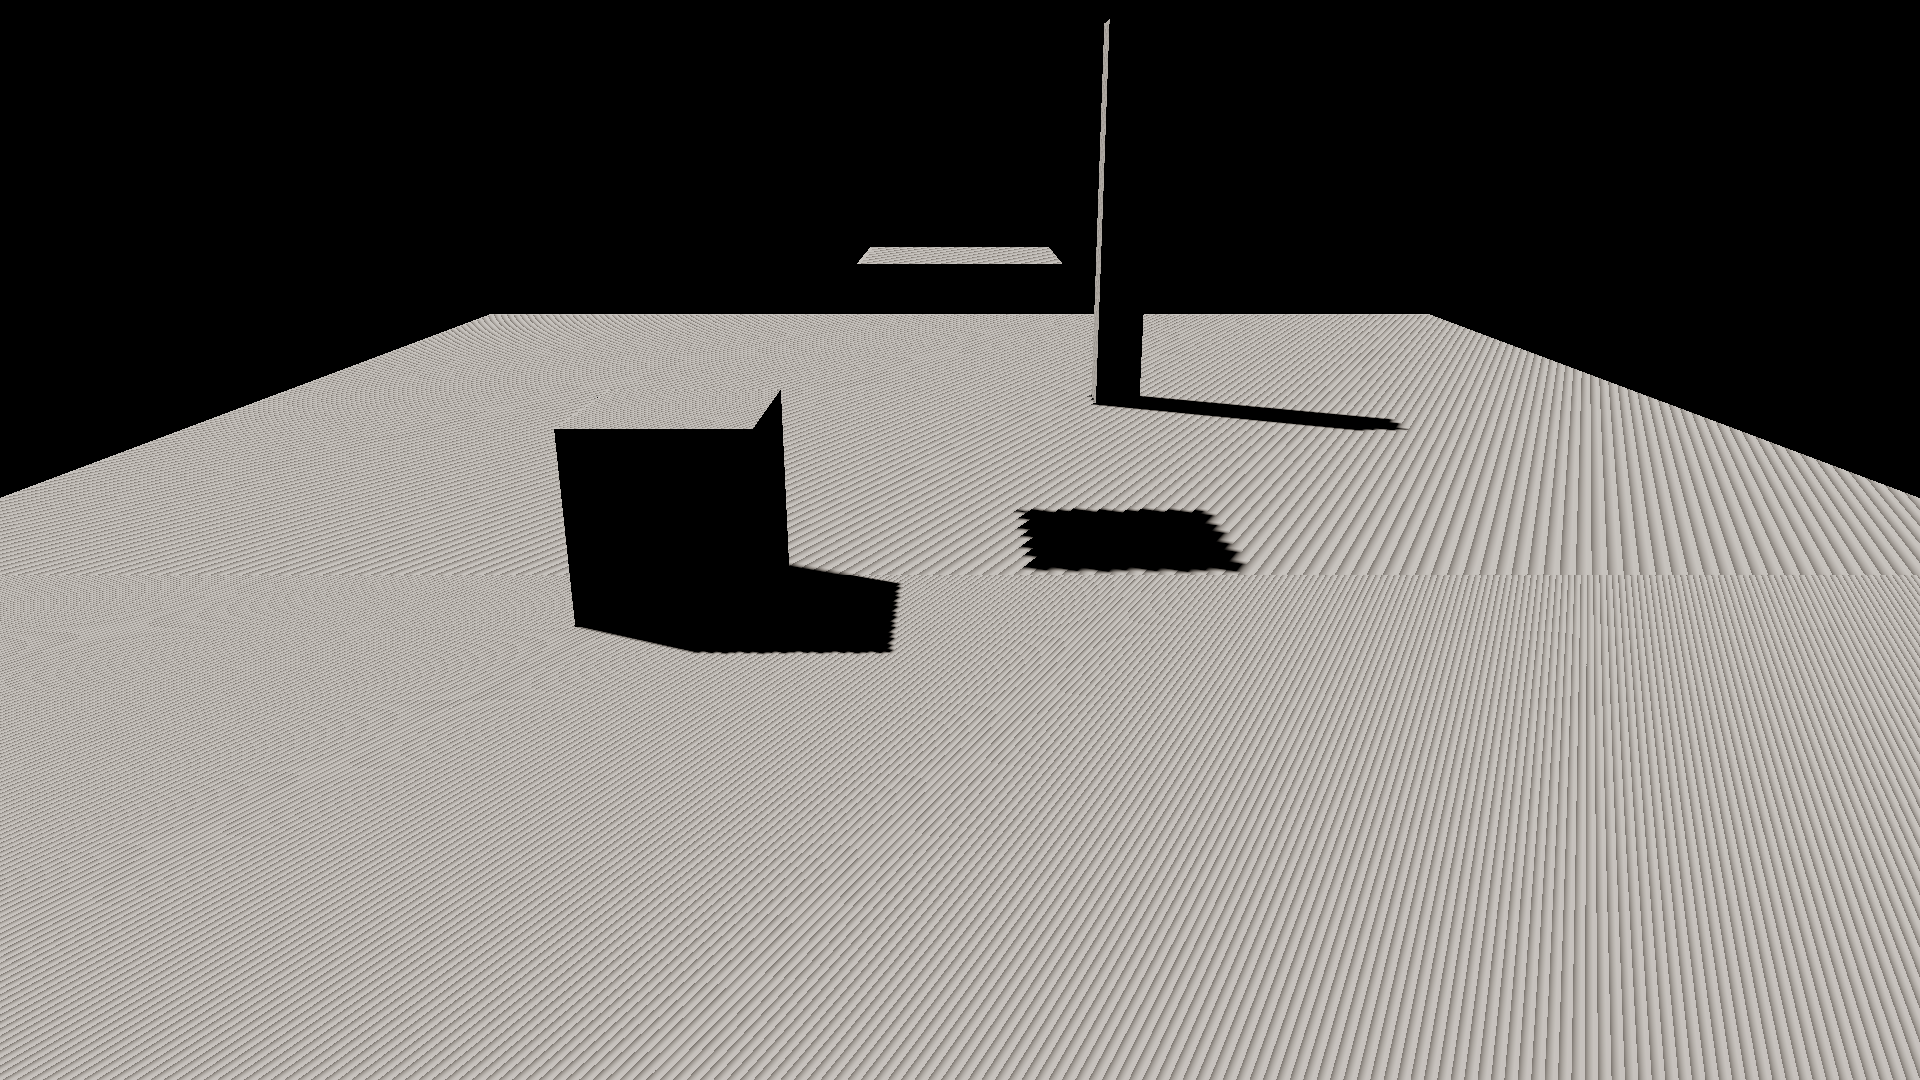
\includegraphics[width=\linewidth]{../../../output/validation/cascaded-shadows/before.png}}{旧版。右下方平地受到沿同一方向排列的假阴影。}\hfill
\panelimage{.485\linewidth}{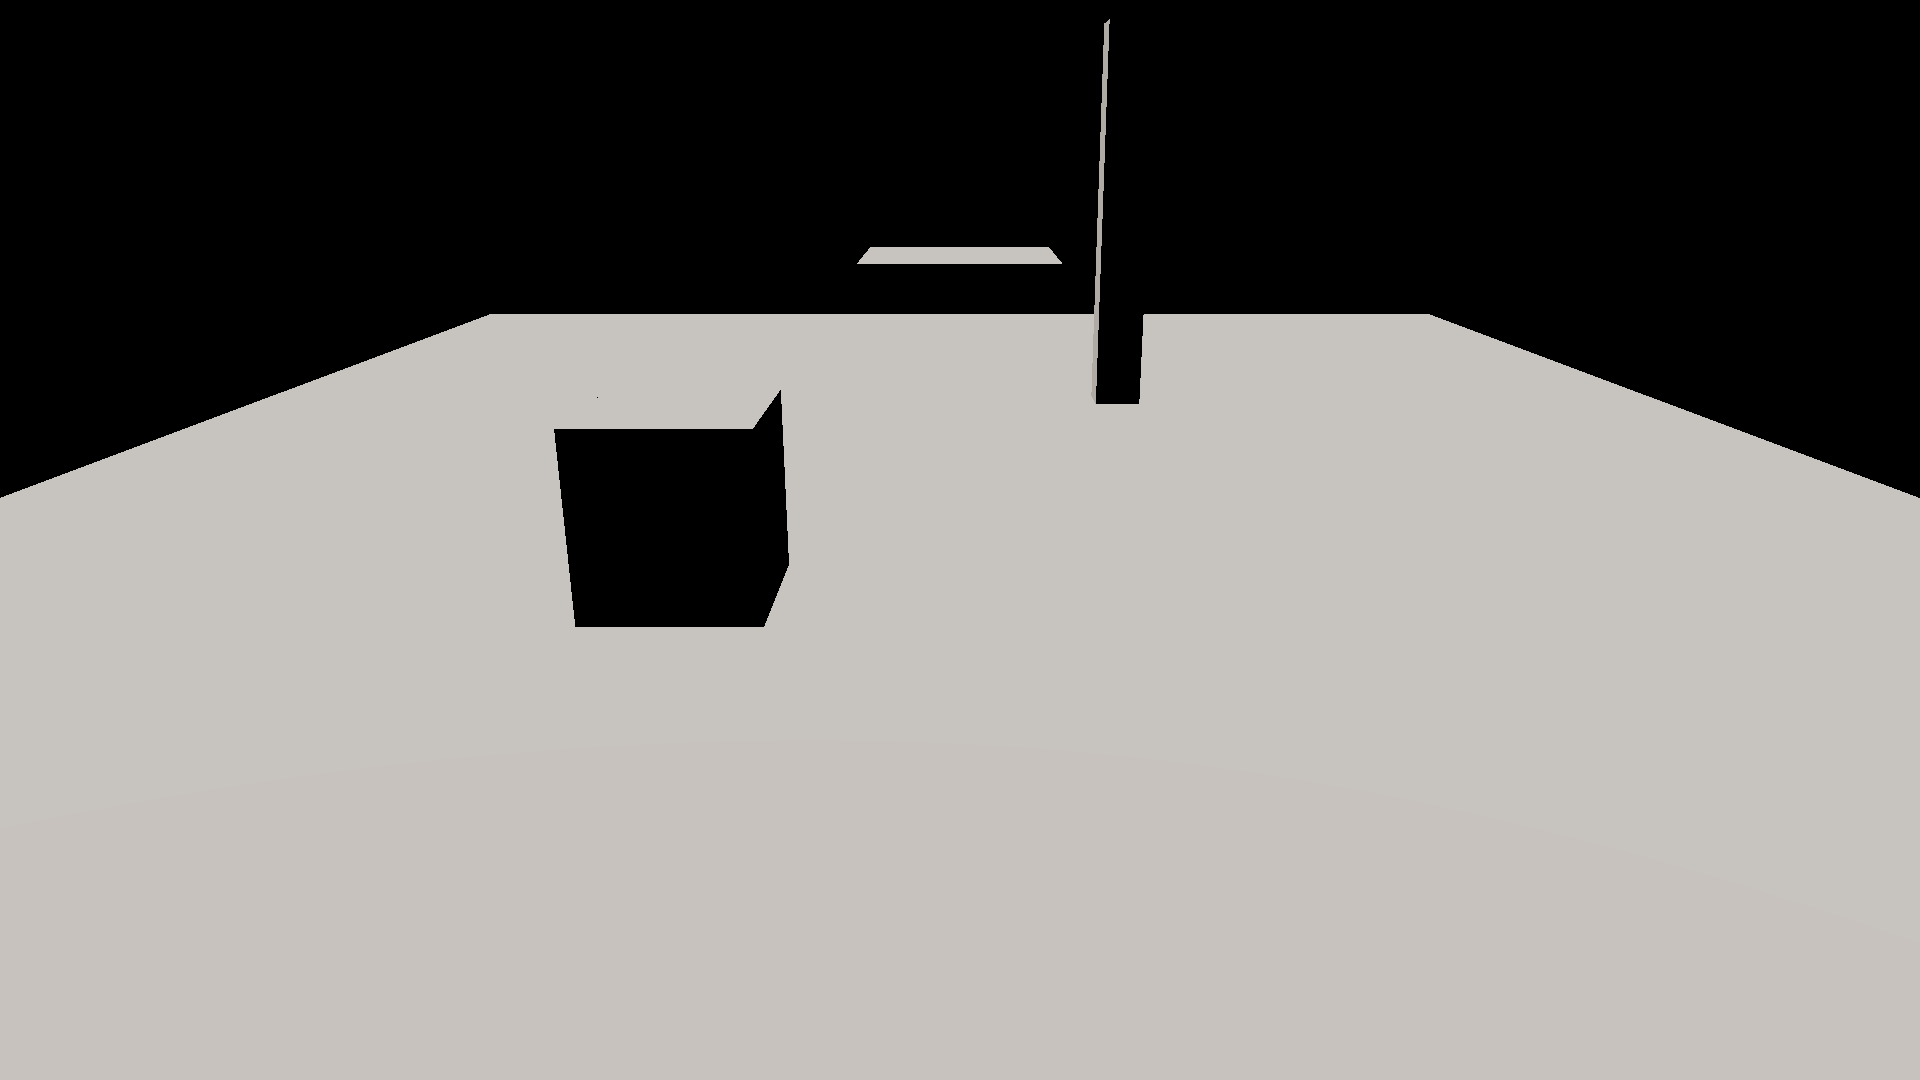
\includegraphics[width=\linewidth]{../../../output/validation/cascaded-shadows/sun-off.png}}{保持灯光强度，关闭投影。两幅均为正式游戏主相机。}
\end{center}

画好的深度图可以沿用到相机、几何或灯光变化。下表上半部是固定游戏相机的第 8 帧，三张图在之前的帧里已经画好。下半部是单独截取重新绘制三张图的过程，三块挡板每层各画一次。两次都用 RTX 5070 Ti Laptop GPU、Debug 构建和 RenderDoc 1.47，预热一次，逐个读 11 次回放事件，表中为中位数。

{\smalltable\noindent\begin{tabularx}{\linewidth}{@{}Xrr@{}}\toprule
工作 & 事件 & GPU 毫秒\\\midrule
游戏直接光，关闭方向光投影 & 66 & 0.287\\
同机位，$0^\circ$ 太阳 & 66 & 0.304\\
同机位，$4^\circ$ 太阳 & 66 & 0.340\\\midrule
独立夹具，九次绘制三块挡板 & 11--95 中的九次绘制 & 0.0054\\
保存三层深度 & 33、70、107 & 0.0135\\
沿三条线读取 771 个地面点 & 119 & 0.0053\\\bottomrule
\end{tabularx}}

在同一夹具中关闭截帧，按一层、三层、三层、一层的顺序测试。每组先画 3 次，随后计时 15 次。同一层数共 30 次。CPU 在回调里给三块挡板记录绘制命令，一层用 0.028 毫秒，三层用 0.085 毫秒。整个 \code{VulkanCascadeMaps::Draw} 从进入到返回分别用 0.279 和 0.827 毫秒。后两项包含 \code{ImmediateSubmit} 等待 GPU 完成的时间。当前每层分别提交绘制与深度保存；将这两步和多层一起记录是下一项可测的改动。

本实现用最多 $5\times5$ 个候选深度估算遮挡物距离，再取至多 $5\times5$ 个点计算半影。搜索半径最多为 16 个阴影像素，宽于它的半影会被截短。三层 $512^2$ 深度数据约占 3 MiB，另需绘制时的暂用图像。级联目前服务于 Vulkan 相机能看到的直接光；探针烘焙继续沿场景的三角形寻找遮挡物，OpenGL 仍使用原来的单张方向光阴影图。

\readings{\refitem{https://learn.microsoft.com/en-us/windows/win32/dxtecharts/cascaded-shadow-maps}{Microsoft，Cascaded Shadow Maps，分层与按相邻纹素修正接收深度}。\refitem{https://developer.download.nvidia.com/shaderlibrary/docs/shadow_PCSS.pdf}{Fernando，Percentage-Closer Soft Shadows，第 3 节及补充图}。源码见 \path{ShadowCascades.cpp}、\path{VulkanCascadeMaps.cpp} 与 \path{GI/Shaders/CascadeVisibility.glsl}。}
